% Author: Izaak Neutelings (October 2021)
% Inspiration
%   "Very special relativity - An illustrated guide", Sander Bais (2007)
\documentclass[border=3pt,tikz]{standalone}
\usepackage{tikz}
\usepackage{amsmath} % for \text
\usepackage{etoolbox} % ifthen
\usepackage[outline]{contour} % glow around text
\usetikzlibrary{decorations.markings,decorations.pathmorphing}
\usetikzlibrary{angles,quotes} % for pic (angle labels)
\usetikzlibrary{arrows.meta} % for arrow size
\usepackage{xfp} % higher precision (16 digits?)
\contourlength{1.1pt}

\newcommand{\calI}{\mathscr{I}} %\mathcal
\tikzset{>=latex} % for LaTeX arrow head
\colorlet{myred}{red!80!black}
\colorlet{myblue}{blue!80!black}
\colorlet{mygreen}{green!80!black}
\colorlet{mydarkred}{red!55!black}
\colorlet{mydarkblue}{blue!50!black}
%\colorlet{mylightblue}{blue!60!black!30}
\colorlet{mypurple}{blue!40!red!80!black}
\colorlet{mydarkgreen}{green!50!black}
\colorlet{mydarkpurple}{blue!40!red!50!black}
%\colorlet{mylightpurple}{mydarkpurple!80!red!6}
\colorlet{myorange}{orange!40!yellow!95!black}
\colorlet{mydarkorange}{orange!40!yellow!85!black}
\tikzstyle{world line}=[myblue!60,line width=0.4]
\tikzstyle{world line t}=[mypurple!60,line width=0.4]
\tikzstyle{world line'}=[mydarkred!60,line width=0.4]
\tikzstyle{mysmallarr}=[-{Latex[length=3,width=2]},thin]
\tikzstyle{mydashed}=[dash pattern=on 3 off 3]
\tikzstyle{vector}=[->,line width=1,line cap=round]
\tikzstyle{vector'}=[vector,shorten >=1.2]
%\tikzstyle{measure}=[{Latex[length=3,width=2]}-{Latex[length=3,width=2]},thin]
\tikzstyle{particle}=[mygreen,line width=0.9]
\tikzstyle{photon}=[-{Latex[length=5,width=4]},myorange,line width=0.8,decorate,
                    decoration={snake,amplitude=1.0,segment length=5,post length=5}]

\def\tick#1#2{\draw[thick] (#1) ++ (#2:0.06) --++ (#2-180:0.12)}
\def\tickp#1#2{\draw[thick,mydarkred] (#1) ++ (#2:0.06) --++ (#2-180:0.12)}
\def\Nsamples{40} % number samples in plot

\begin{document}

% SPACETIME DIAGRAM - LORENTZ BOOST
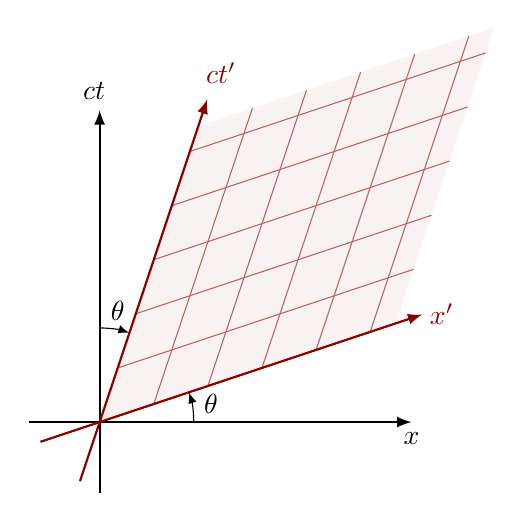
\begin{tikzpicture}[scale=1.8]
  \message{Lorentz boost^^J}
  
  \def\xmax{2}
  \def\xmaxp{2.2} % maximum of rotated axis
  \def\Nlines{5} % number of world lines (at constant x/t)
  \pgfmathsetmacro\ang{atan(1/3)} % angle between x and x' axes
  \pgfmathsetmacro\d{0.9*\xmax/\Nlines} % grid size
  \pgfmathsetmacro\D{\d/cos(\ang)/sqrt(1-tan(\ang)^2)} % grid size, boosted
  \coordinate (O) at (0,0);
  \coordinate (X) at (\xmax+0.2,0);
  \coordinate (T) at (0,\xmax+0.2);
  \coordinate (X') at (\ang:\xmaxp+0.2);
  \coordinate (T') at (90-\ang:\xmaxp+0.2);

  
  % BOOSTED WORLD LINE GRID
  \message{Making world lines for boosted frame...^^J}
  \fill[mydarkred,opacity=0.05]
    (O) --++ (\ang:\xmaxp) --++ (90-\ang:\xmaxp) --++ (\ang:-\xmaxp) -- cycle;
  \foreach \i [evaluate={\x=\i*\D;}] in {1,...,\Nlines}{
    \message{  Running i/N=\i/\Nlines, x=\x...^^J}
    \draw[world line'] (\ang:\x) --++ (90-\ang:\xmaxp);
    \draw[world line'] (90-\ang:\x) --++ (\ang:\xmaxp);
  }
  
  % AXES
  \draw[->,thick] (0,-0.5) -- (T) node[left=2, above=0] {$ct$};
  \draw[->,thick] (-0.5,0) -- (X) node[below=0] {$x$};
  \draw[->,thick,mydarkred] (90-\ang:-0.2*\xmaxp) -- (T')
    node[right=5,above=2] {$ct'$};
  \draw[->,thick,mydarkred] (\ang:-0.2*\xmaxp) -- (X') node[right=-1] {$x'$};
  
  % ANGLES
  \draw pic[->,"$\theta$",draw=black,angle radius=34,angle eccentricity=1.2] {angle = X--O--X'};
  \draw pic[<-,"$\theta$",draw=black,angle radius=34,angle eccentricity=1.2] {angle = T'--O--T};
  
\end{tikzpicture}

% SPACETIME DIAGRAM - LORENTZ BOOST
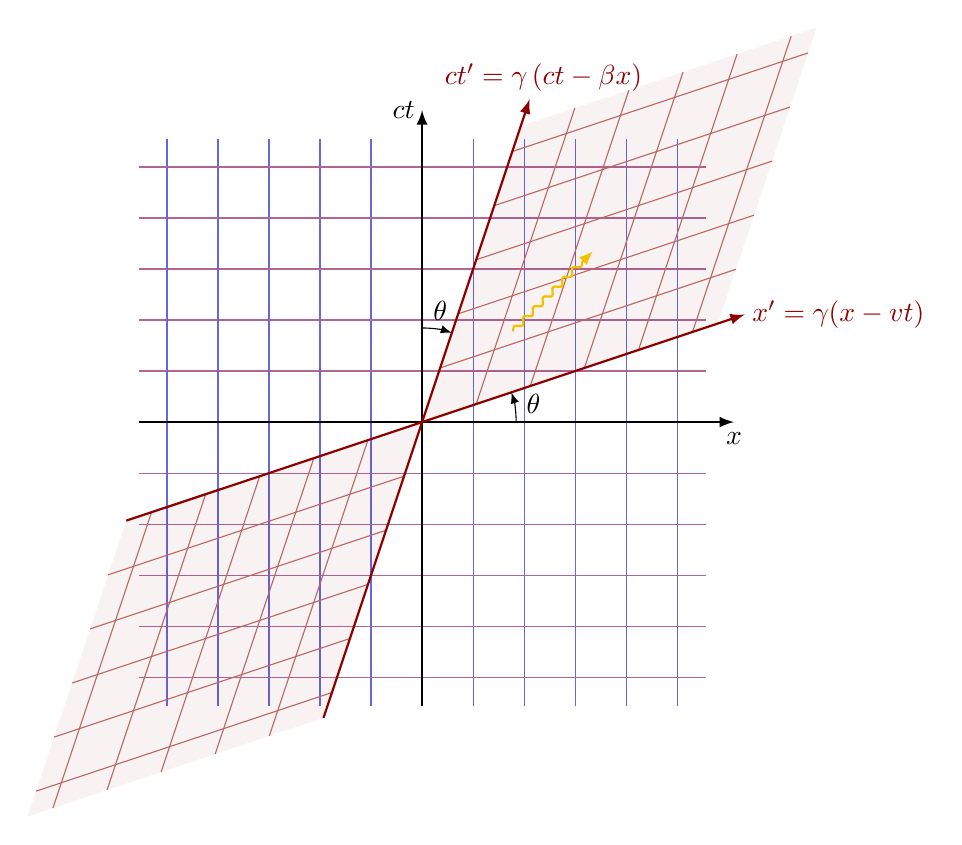
\begin{tikzpicture}[scale=1.8]
  \message{Lorentz boost^^J}
  
  \def\xmax{2}
  \def\xmaxp{2.2} % maximum of rotated axis
  \def\Nlines{5} % number of world lines (at constant x/t)
  \pgfmathsetmacro\ang{atan(1/3)} % angle between x and x' axes
  \pgfmathsetmacro\d{0.9*\xmax/\Nlines} % grid size
  \pgfmathsetmacro\D{\d/cos(\ang)/sqrt(1-tan(\ang)^2)} % grid size, boosted
  \coordinate (O) at (0,0);
  \coordinate (X) at (\xmax+0.2,0);
  \coordinate (T) at (0,\xmax+0.2);
  \coordinate (X') at (\ang:\xmaxp+0.2);
  \coordinate (T') at (90-\ang:\xmaxp+0.2);
  
  % WORLD LINE GRID
  \message{Making world lines...^^J}
  \foreach \i [evaluate={\x=\i*\d;}] in {1,...,\Nlines}{
    \message{  Running i/N=\i/\Nlines, x=\x...^^J}
    \draw[world line]   (-\x,-\xmax) -- (-\x,\xmax);
    \draw[world line]   ( \x,-\xmax) -- ( \x,\xmax);
    \draw[world line t] (-\xmax,-\x) -- (\xmax,-\x);
    \draw[world line t] (-\xmax, \x) -- (\xmax, \x);
  }
  
  % BOOSTED WORLD LINE GRID
  \message{Making world lines for boosted frame...^^J}
  \fill[mydarkred,opacity=0.05]
    (O) --++ (\ang:\xmaxp) --++ (90-\ang:\xmaxp) --++ (\ang:-\xmaxp) -- cycle;
  \fill[mydarkred,opacity=0.05]
    (O) --++ (\ang:-\xmaxp) --++ (90-\ang:-\xmaxp) --++ (\ang:\xmaxp) -- cycle;
  \foreach \i [evaluate={\x=\i*\D;}] in {1,...,\Nlines}{
    \message{  Running i/N=\i/\Nlines, x=\x...^^J}
    \draw[world line'] (\ang:-\x) --++ (90-\ang:-\xmaxp);
    \draw[world line'] (90-\ang:-\x) --++ (\ang:-\xmaxp);
    \draw[world line'] (\ang:\x) --++ (90-\ang:\xmaxp);
    \draw[world line'] (90-\ang:\x) --++ (\ang:\xmaxp);
  }
  
  % AXES
  \draw[->,thick] (0,-\xmax) -- (T) node[left=-1] {$ct$};
  \draw[->,thick] (-\xmax,0) -- (X) node[below=0] {$x$};
  \draw[->,thick,mydarkred] (90-\ang:-\xmaxp) -- (T')
    node[right=5,above=-1] {$ct' = \gamma\left(ct-\beta x\right)$};
  \draw[->,thick,mydarkred] (\ang:-\xmaxp) -- (X') node[right=-1] {$x' = \gamma(x-vt)$};
  
  % ANGLES
  \draw pic[->,"$\theta$",draw=black,angle radius=34,angle eccentricity=1.2] {angle = X--O--X'};
  \draw pic[<-,"$\theta$",draw=black,angle radius=34,angle eccentricity=1.2] {angle = T'--O--T};
  
  % PHOTON
  \draw[photon] (0.32*\xmax,0.32*\xmax) --++ (45:0.4*\xmax);
  
\end{tikzpicture}


\end{document}